This chapter describes the implementation of the smartphone app and the different decisions made during this phase of the development. 

\section{Target Platform}
The first decision we had to make was which platforms to target. This decision has an impact on the potential userbase of the app. It is not ideal if potential users are kept from using our system due to the platforms it is available on.
The two main platforms we considered developing for is Android and IOS. To facilitate development for both platforms we decided on using Xamarin \cite{xamarin} as our development platform. 
Xamarin is a development platform designed with cross-platform app development in mind. 
It enables reuse of significant parts of the code, thus cutting down the potential development time needed to develop for multiple platforms. Some platform-specific code is still necessary for performing platform specific actions, like performing visual actions that is not handled through the Xamarin framework, and setting up permissions specifically for each platform.
The individual platforms has dedicated IDE’s each(XCode\cite{xcode} for IOS, and Android Studio for Android), but none of those can facilitate the same cross-platform development that Xamarin can. 
The development of a full app for both platforms is however not the focus of this project, and as such we will only develop for Android as a sort of proof of concept. Development will still be done using Xamarin. 

\section{Libraries used}
We are using a few different libraries in the android version of the app. We chose to use these libraries to speed up the development process, and to help implement things in a proper way.
\begin{itemize}
    \item Rendy Del Rosario/FirebasePushNotificationPlugin
    \item Wilson Vargas/ButtonCircle
    \item Xamarin additional libraries
    \item dsplaisted/PCLStorage
\end{itemize}

ButtonCircle is a simple library for creating a round button.
PCLStorage is a cross platform library for handling file IO on various mobile platforms - including Android and IOS. While an android specific library (or native android functionality) could have been used, we decided to use PCLStorage to prepare for future development on a different platform.

\section{Server communication}
Communication with the backend of the system is done through a Rest-API. 
\begin{figure}[h]
    \centering
    \begin{lstlisting}

    HttpWebRequest request = (HttpWebRequest) HttpWebRequest.Create(url);
    request.Method = "GET";
    request.Headers.Add("email", UsernameText);
    request.Headers.Add("password", PasswordText);

    using (var response = request.GetResponse())
    {
        switch (((HttpWebResponse)response).StatusCode)
        {
            case HttpStatusCode.OK:
                using (var reader = new StreamReader(response.GetResponseStream()))
                {
                    string json = reader.ReadToEnd();
                    json = JsonConvert.DeserializeObject<dynamic>(json) ["body"].ToString();
                    currentUser = JsonConvert.DeserializeObject<User>(json);
                    currentUser.jsonCredentials = json;

                    if (currentUser.contacts == null && currentUser.id != -1)
                    {
                        CreateUserCredentialsFile(currentUser);
                        return true;
                    }

                    currentUser.setNumber();
                }
                if (currentUser.id != -1)
                {
                    CreateUserCredentialsFile(currentUser);
                    return true;
                }
                break;

            default:
                CrossPlatFormMethod.WriteTextToScreen("Kunne ikke forbinde til serveren.");
                return false;
        }
    }
\end{lstlisting}
    \caption{Login in to the server}
    \label{fig:appLogIn}
\end{figure}
In the figure \ref{fig:appLogIn} we have an example of the login \textit{GET} request that returns a citizen/contact. When a successful request is made, the recieved object is then deserialized. First, it is converted to an object of type dynamic, containing only the body of the JSON object, since the only part of the response object we are interested in is the body. The next step is then then to deserialize the content of the body into our model of a user. Seperate checks are made to find out whether or not a user has a phonenumber or not, and if they do, an additional deserialization is made to save the phonenumber.

\section{Firebase Cloud Messaging}
We use Firebase Cloud Messaging(FCM) which is developed by Google to facilitate the usage of push notifications on android. FCM works by utilizing a background service, which watches for new messages. The setup for FCM specifically gave us some troubles during the development. Before trying to use FCM, we tried to setup an older solution from google, Google Cloud Messaging (GCM). GCM however, proved difficult to setup. Due to this, and the amount of time that was spent on trying to make it work, it was decided to use FCM and a library instead. The library (FirebasePushNotificationPlugin by Rendy Del Rosario \todo{ref}) handles most of the setup involved in using FCM.

FCM handles user registration using tokens, which we then store on the server-side whenever a token refresh or creation happens.

\section{Cross Platform}
We chose to use Xamarin since this allowed us to make it easier to create the app for both android and IOS. But, even though Xamarin allows for code reuse between platforms, we still need platform specific code in some cases. This is done through a class we created called \textit{CrossPlatformMethod}, which contains a set of static methods allowing us to perform certain actions without having to consider how to do it on each platform, thus making it cross-platform. Each method then implements a version of the code that is compiled down to each platform. In our case, only the Android part is actually implemented, since that is the only platform we are developing for in this project. 

\begin{figure}[h]
    \centering
    \begin{lstlisting}
    public static void WriteTextToScreen(string message)
    {
        #if __ANDROID__
            Toast.MakeText(Xamarin.Forms.Forms.Context, message, ToastLength.Long).Show();
        #elif IOS
        #endif
    }
    \end{lstlisting}
    \caption{Multi pathform code}
    \label{fig:appMultiPlatform}
\end{figure}
In figure \ref{fig:appMultiPlatform} we use directives to say tell the compiler what part of the code it should compile down to the different platforms. We have only implemented the app for Android, but having a class like \ref{fig:appMultiPlatform} makes it easier to implement the app on IOS in the future.

\section{MVVM Pattern}
We are using the MVVM(Model View ViewModel) pattern so that we can separate the view design and the code-behind to make it easier to maintain and change things down the line. It also lets us work on views and viewmodels concurrently, and therefore speeds up the development process. These elements (models, views and viewmodels) are created so that they can be reused for all platforms. The usage of MVVM does have some side effects, as it forces us to work with screens differently from what is normally done on the android platform. One specific example is that the back button on an android phone does not work to navigate between the different screens, due to the fact that in native android a views are normally separate activities, which they are not in our MVVM model.



\section{Usability}
The usability of the app is not a very important part of this project. It is however still designed with disoriented/elderly people in mind. 

\begin{figure}
    \centering
    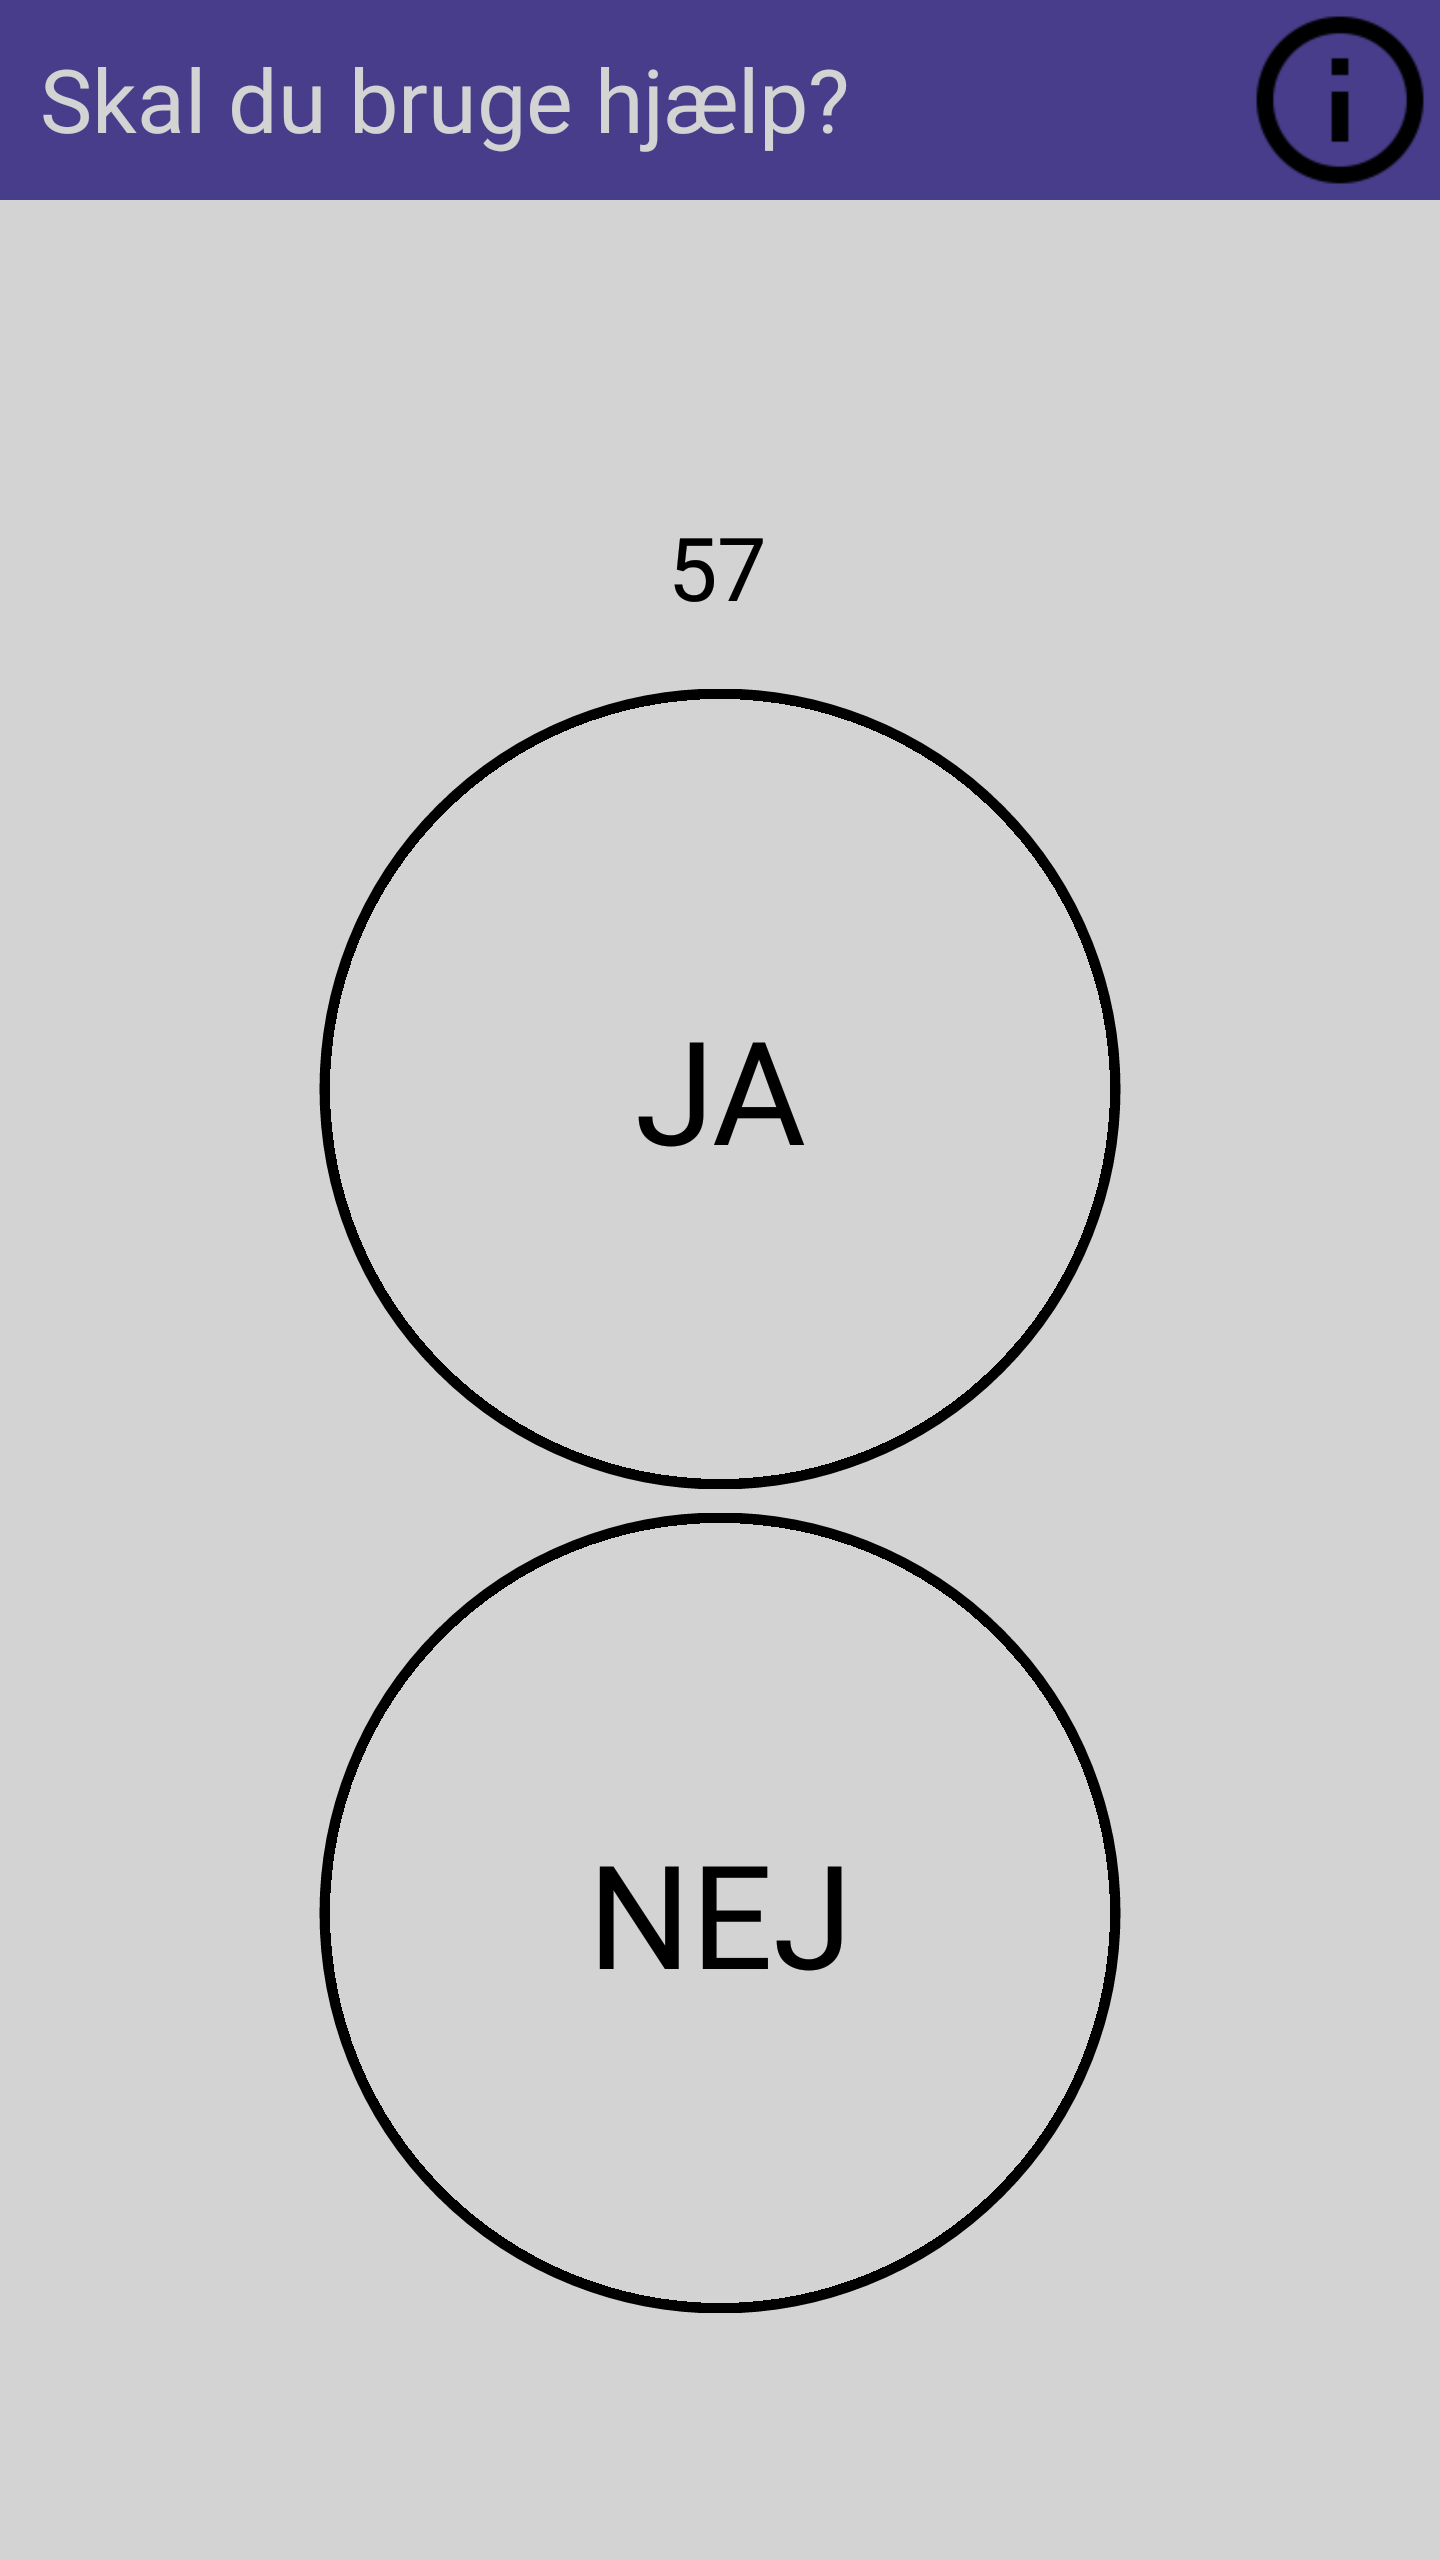
\includegraphics[scale=0.1]{Figures/usabapp.png}
    \caption{Caption}
    \label{fig:usabapp}
\end{figure}


On \ref{fig:usabapp} is the screen a user of the system is presented with when confirming or aborting a call for help. The buttons and text are made large on purpose, to make it easier for the target audience to see and use the buttons. Other than this, no usability testing has been performed, as it is not the main focus of this project.